\section{Résultats}
\label{sec:resultats}

Ce chapitre présente les résultats bruts de l'essai, sans les interpréter~: leur analyse et leur comparaison avec les valeurs du constructeur font l'objet du chapitre suivant. Toutes les valeurs relevées sont rassemblées dans les tableaux de l'annexe~\ref{subsec:valeurs}.

\subsection{Déroulement de l'essai}
\label{subsec:deroulement}

L'essai a duré 115~minutes, avec un relevé toutes les 5~minutes. À 0~min, la cogénération est à l'arrêt~: ce premier relevé donne les conditions initiales (index des compteurs, température de l'eau et de l'air ambiant, fumées à 21\,\% d'O\textsubscript{2}). Elle démarre juste après, puisque les compteurs ont déjà varié au relevé suivant. Les deux radiateurs, fermés au départ, ont été ouverts à tour de rôle pour dissiper de la chaleur (tableau~\ref{tab:evenements}).

\begin{table}[htbp]
  \centering
  \caption{Chronologie de l'essai (relevés)}
  \label{tab:evenements}
  \begin{tabular}{cl}
    \hline
    Temps (min) & Événement \\
    \hline
    0 & Cogénération à l'arrêt, relevé initial \\
    5 & Premier relevé en fonctionnement \\
    65 & Petit radiateur ouvert \\
    75 & Grand radiateur ouvert \\
    95 & Petit radiateur de nouveau fermé \\
    110 & Grand radiateur de nouveau fermé \\
    115 & Dernier relevé \\
    \hline
  \end{tabular}
\end{table}

Les deux radiateurs ont donc été ouverts simultanément entre 75 et 90~min. Dans les graphiques qui suivent, les périodes d'ouverture sont indiquées par des zones colorées.

\subsection{Températures du circuit hydraulique}
\label{subsec:res-temperatures}

\paragraph{Ballon et cuve.} La figure~\ref{fig:temp-ballon} montre l'évolution des températures de l'eau dans le ballon. À l'entrée du ballon, la température passe de 20,5 à 56,8\,°C en 115~min~; à la sortie, de 18,6 à 48,9\,°C. La montée est lente pendant les 25~premières minutes (de 29,5 à 31,6\,°C à l'entrée entre 5 et 25~min), puis s'accélère à partir de 30~min. L'écart entre l'entrée et la sortie du ballon est compris entre 7,9 et 11,1\,K (moyenne de 9,6\,K) pendant l'essai. La température de la cuve passe de 15,7 à 49,4\,°C. La température en sortie de cuve n'a été relevée qu'à partir de 30~min~: elle passe de 28 à 50\,°C, avec un maximum de 52\,°C. La limite de 60\,°C, à laquelle la cogénération s'arrête (section~\ref{subsec:utilisation}), n'a pas été atteinte.

\begin{figure}[htbp]
  \centering
  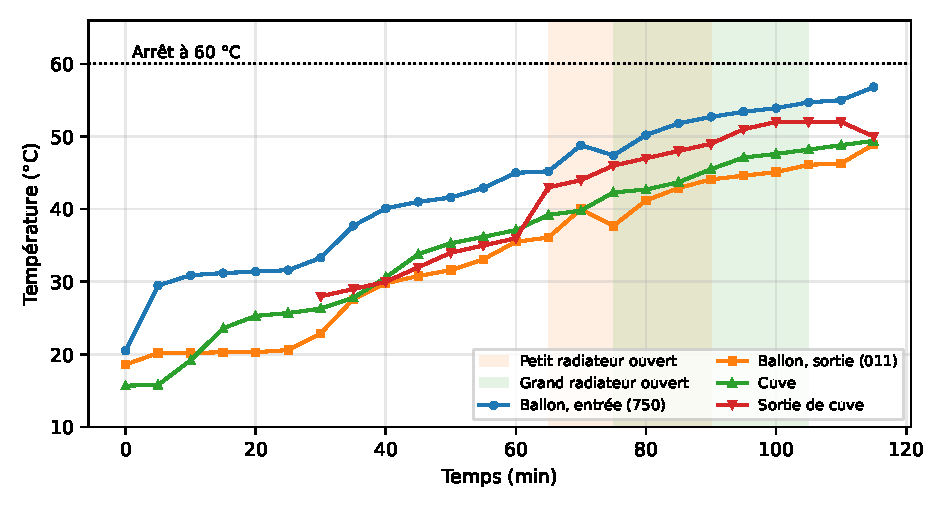
\includegraphics[width=0.9\textwidth]{Images/res_temp_ballon.pdf}
  \caption{Évolution des températures du ballon et de la cuve}
  \label{fig:temp-ballon}
\end{figure}

\paragraph{Radiateurs.} Les températures des radiateurs sont représentées à la figure~\ref{fig:temp-radiateurs}. Tant qu'ils sont fermés, elles restent à environ 20\,°C, soit la température ambiante au début de l'essai.
\begin{itemize}
  \item \emph{Grand radiateur}~: à l'ouverture (75~min), l'eau arrive à 45,6\,°C à l'entrée alors que la sortie n'est qu'à 27,3\,°C (écart de 18,3\,K), le radiateur étant encore froid. L'écart entre l'entrée et la sortie diminue ensuite de 4,8\,K (80~min) à 2,2\,K (100~min). L'entrée atteint 53,2\,°C à 105~min, puis les températures diminuent après la fermeture (42,9\,°C à l'entrée et 40,9\,°C à la sortie à 115~min).
  \item \emph{Petit radiateur}~: à l'ouverture (65~min), l'entrée est à 39,4\,°C et la sortie à 36,8\,°C (écart de 2,6\,K). Les deux températures montent ensuite ensemble jusqu'à environ 49\,°C à 90~min, avec des valeurs d'entrée et de sortie très proches, la sortie étant même légèrement supérieure à l'entrée (de 0,4 à 1,2\,K d'écart). Après la fermeture, elles redescendent jusqu'à 31,0\,°C à l'entrée et 31,5\,°C à la sortie à 115~min.
\end{itemize}

\begin{figure}[htbp]
  \centering
  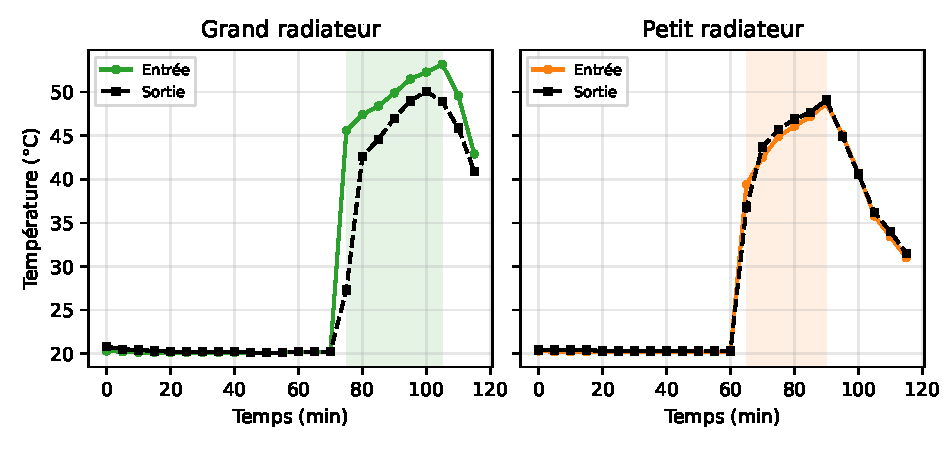
\includegraphics[width=0.95\textwidth]{Images/res_temp_radiateurs.pdf}
  \caption{Températures d'entrée et de sortie des radiateurs}
  \label{fig:temp-radiateurs}
\end{figure}

\subsection{Composition des fumées}
\label{subsec:res-fumees}

Les mesures de l'analyseur Testo~320 sont reprises à la figure~\ref{fig:fumees}. Au relevé initial, la cogénération étant à l'arrêt, l'analyseur indique 21\,\% d'O\textsubscript{2} et 0\,ppm de CO, et le CO\textsubscript{2} n'est pas affiché. En fonctionnement~:
\begin{itemize}
  \item la température des fumées passe de 66,3\,°C (5~min) à environ 70\,°C dès 10~min, puis reste comprise entre 70 et 73\,°C, avec une moyenne de 71,2\,°C~;
  \item la teneur en O\textsubscript{2} est stable à 8,0--8,1\,\% jusqu'à 60~min, puis devient plus variable, entre 8,1 et 11,1\,\%, avec une moyenne de 8,8\,\%~;
  \item la teneur en CO\textsubscript{2}, calculée par l'analyseur à partir de l'O\textsubscript{2}, évolue en sens inverse~: de 8,4\,\% au début, elle descend jusqu'à 6,4\,\%, avec une moyenne de 7,9\,\%~;
  \item la teneur en CO est comprise entre 393 et 588\,ppm, avec une moyenne de 486\,ppm~;
  \item la température ambiante augmente de 22,2 à 29,8\,°C.
\end{itemize}

\begin{figure}[htbp]
  \centering
  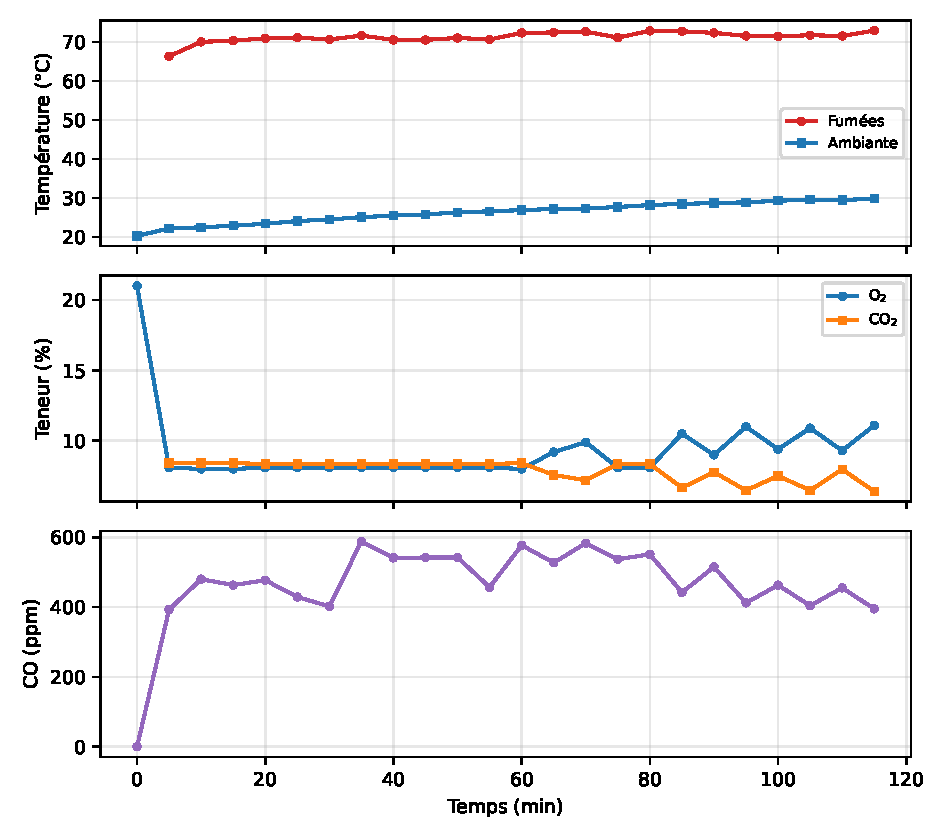
\includegraphics[width=0.9\textwidth]{Images/res_fumees.pdf}
  \caption{Mesures de l'analyseur de combustion Testo~320}
  \label{fig:fumees}
\end{figure}

\subsection{Consommation et production}
\label{subsec:res-puissances}

Les puissances sont déduites des relevés de compteurs et du système d'acquisition (section~\ref{sec:appareils}). Pour un pas de 5~minutes, avec $\Delta V$ la variation d'index du compteur de gaz (en m\textsuperscript{3}) et $\Delta E$ celle du compteur d'électricité (en kWh)~:
\begin{align}
  P_{\mathrm{gaz}} &= 12\,\Delta V \cdot \frac{\rho \cdot \mathrm{PCI}}{3600} \\
  P_{\mathrm{el}} &= 12\,\Delta E \\
  P_{\mathrm{th}} &= \frac{\text{Heat power}}{3{,}6}
\end{align}
avec $P_{\mathrm{gaz}}$, $P_{\mathrm{el}}$ et $P_{\mathrm{th}}$ en kW, et \emph{Heat power} la puissance thermique récupérée fournie par l'acquisition, en MJ/h. Pour le gaz naturel, nous avons pris une masse volumique $\rho$ de 0,7\,kg/m\textsuperscript{3} et un pouvoir calorifique inférieur PCI de 50\,MJ/kg (soit 35\,MJ/m\textsuperscript{3}, ou environ 9,7\,kWh/m\textsuperscript{3}).

Sur les 115~minutes de l'essai, la cogénération a consommé 4,442\,m\textsuperscript{3} de gaz (environ 43,2\,kWh), produit 10,59\,kWh d'électricité et récupéré environ 17,7\,kWh de chaleur. L'évolution des puissances est représentée à la figure~\ref{fig:puissances}~:
\begin{itemize}
  \item la puissance du gaz consommé est de 22,5\,kW en moyenne (de 17,4 à 26,5\,kW), pour un débit moyen de 2,32\,m\textsuperscript{3}/h~;
  \item la puissance thermique récupérée est stable, sans tendance au cours de l'essai, avec une moyenne de 9,2\,kW (de 8,3 à 10,4\,kW)~;
  \item la puissance électrique, déduite du compteur, varie davantage d'un relevé à l'autre, de 3,5 à 7,3\,kW, avec une moyenne de 5,5\,kW.
\end{itemize}
La puissance électrique de sortie (\emph{W out}) affichée par le système d'acquisition est quant à elle restée à 6\,000\,W à chaque relevé en fonctionnement.

\begin{figure}[htbp]
  \centering
  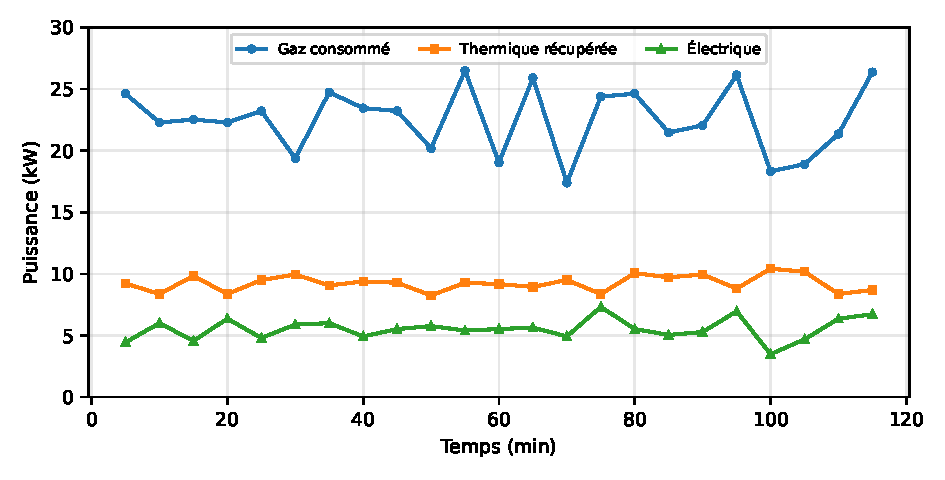
\includegraphics[width=0.9\textwidth]{Images/res_puissances.pdf}
  \caption{Puissances du gaz consommé, thermique récupérée et électrique}
  \label{fig:puissances}
\end{figure}

\subsection{Rendements}
\label{subsec:res-rendements}

Les rendements sont calculés pour chaque pas de 5~minutes, en rapportant les puissances électrique et thermique à celle du gaz consommé~:
\begin{equation}
  \eta_{\mathrm{el}} = \frac{P_{\mathrm{el}}}{P_{\mathrm{gaz}}}, \qquad
  \eta_{\mathrm{th}} = \frac{P_{\mathrm{th}}}{P_{\mathrm{gaz}}}, \qquad
  \eta_{\mathrm{global}} = \eta_{\mathrm{el}} + \eta_{\mathrm{th}}
\end{equation}
Leur évolution est représentée à la figure~\ref{fig:rendements} et leurs valeurs moyennes, sur les relevés de 5 à 115~min, sont reprises dans le tableau~\ref{tab:rendements}. Les valeurs instantanées fluctuent d'un relevé à l'autre, car elles dépendent de la variation d'index de compteurs relevés manuellement sur un pas de seulement 5~minutes.

\begin{table}[htbp]
  \centering
  \caption{Rendements mesurés (moyenne sur 5 à 115~min)}
  \label{tab:rendements}
  \begin{tabular}{lccc}
    \hline
    Rendement & Moyenne (\%) & Minimum (\%) & Maximum (\%) \\
    \hline
    Électrique & 24,7 & 18,0 & 30,4 \\
    Thermique & 41,8 & 33,0 & 56,9 \\
    Global & 66,4 & 55,4 & 83,0 \\
    \hline
  \end{tabular}
\end{table}

\begin{figure}[htbp]
  \centering
  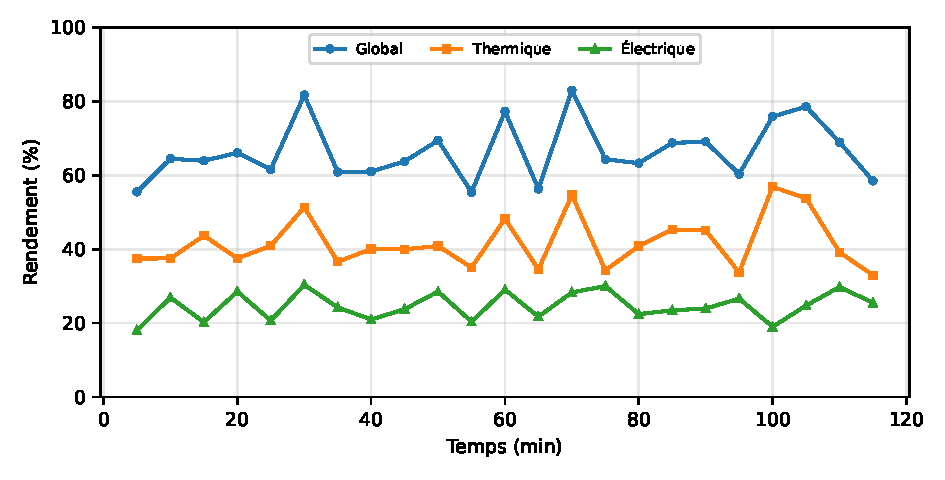
\includegraphics[width=0.9\textwidth]{Images/res_rendements.pdf}
  \caption{Évolution des rendements électrique, thermique et global}
  \label{fig:rendements}
\end{figure}
